\documentclass{standalone}
\usepackage{graphicx}	
\usepackage{amssymb, amsmath}
\usepackage{color}

\usepackage{tikz}
\usetikzlibrary{intersections, backgrounds, patterns, patterns.meta}
\usepackage{pgfmath}

\definecolor{light}{RGB}{220, 188, 188}
\definecolor{mid}{RGB}{185, 124, 124}
\definecolor{dark}{RGB}{143, 39, 39}
\definecolor{highlight}{RGB}{180, 31, 180}
\definecolor{gray10}{gray}{0.1}
\definecolor{gray20}{gray}{0.2}
\definecolor{gray30}{gray}{0.3}
\definecolor{gray40}{gray}{0.4}
\definecolor{gray60}{gray}{0.6}
\definecolor{gray70}{gray}{0.7}
\definecolor{gray80}{gray}{0.8}
\definecolor{gray90}{gray}{0.9}
\definecolor{gray95}{gray}{0.95}

\begin{document}

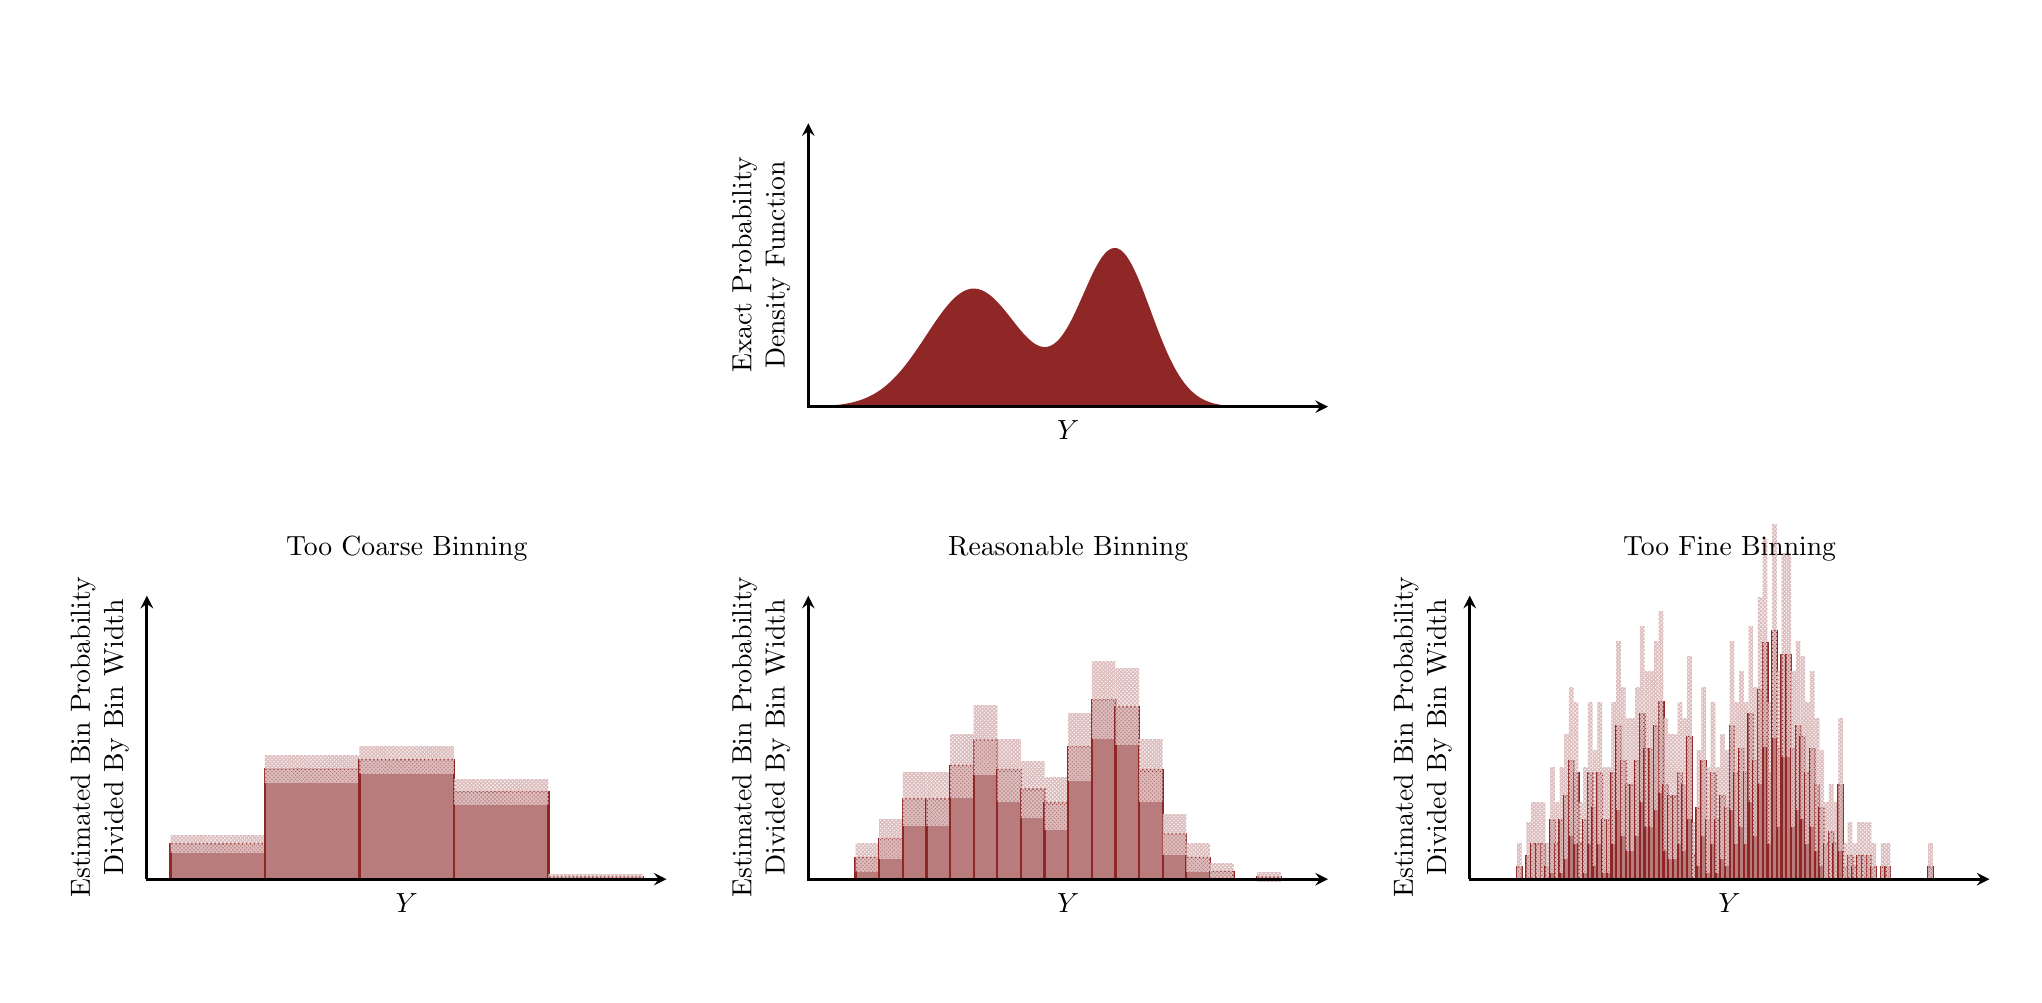
\begin{tikzpicture}[scale=0.3, thick]

\pgfmathsetmacro{\hscale}{2};
\pgfmathsetmacro{\vscale}{30};

\begin{scope}[shift={(0, 0)}]
  \draw[white] (-16, -4) rectangle (12, 16);

  \fill[domain={-5:5}, smooth, samples=150, line width=1, variable=\x, color=dark] 
    plot ({\hscale * \x},{5 * (exp(-0.5 * (\x - 1) * (\x - 1) / (0.75 * 0.75) ) / 0.75 + exp(-0.5 * (\x + 2) * (\x + 2) / (1 * 1) ) / 1)});
  
  \draw [->, >=stealth, line width=1] (-11, 0) -- (-11, 12);
  \node[rotate=90, align=center] at (-13, 6) { Exact Probability\\Density Function };
  
  \draw [->, >=stealth, line width=1] (-11.05, 0) -- (11, 0);
  \node at (0, -1) { $Y$ };
\end{scope}

\begin{scope}[shift={(-28, -20)}]
  \draw[white] (-16, -4) rectangle (12, 16);

  \foreach \p [count=\n] in {0.1, 0.311666666666667, 0.336666666666667, 0.245, 0.00666666666666667} {
    \pgfmathsetmacro{\yl}{-5 + 2 * (\n - 1)};
    \pgfmathsetmacro{\yu}{-5 + 2 * \n};  
    
    \pgfmathsetmacro{\vertscale}{\vscale / 2};  
    
    \filldraw[fill=mid, draw=dark] (\hscale * \yl, 0) rectangle (\hscale * \yu, \vertscale * \p);
    
    \pgfmathsetmacro{\delta}{2 * sqrt(\p * (1 - \p)) * 0.040824829046386};  
    
    \fill[pattern={Hatch[angle=45,distance=1, line width=0.5]}, pattern color=light] 
      (\hscale * \yl, {\vertscale * (\p - \delta)}) rectangle (\hscale * \yu, {\vertscale * (\p + \delta)});
  }

  \draw [->, >=stealth, line width=1] (-11, 0) -- (-11, 12);
  \node[rotate=90, align=center] at (-13, 6) { Estimated Bin Probability\\Divided By Bin Width };
  
  \node at (0, 14) { Too Coarse Binning };
  \draw [->, >=stealth, line width=1] (-11.05, 0) -- (11, 0);
  \node at (0, -1) { $Y$ };
\end{scope}

\begin{scope}[shift={(28, -20)}]
  \draw[white] (-16, -4) rectangle (12, 16);

  \foreach \p [count=\n] in {0, 0, 0, 0, 0, 0.00166666666666667, 0, 0.00333333333333333, 
                             0.005, 0.005, 0.005, 0.00166666666666667, 0.00833333333333333, 
                             0.005, 0.00833333333333333, 0.0116666666666667, 0.0166666666666667, 
                             0.015, 0.005, 0.00833333333333333, 0.015, 0.01, 0.015, 
                             0.00833333333333333, 0.00833333333333333, 0.015, 0.0216666666666667, 
                             0.0166666666666667, 0.0133333333333333, 0.0133333333333333, 
                             0.0166666666666667, 0.0233333333333333, 0.0183333333333333, 
                             0.0183333333333333, 0.0216666666666667, 0.025, 0.0133333333333333, 
                             0.0116666666666667, 0.0116666666666667, 0.015, 0.0133333333333333, 
                             0.02, 0.00333333333333333, 0.01, 0.0166666666666667, 0.00833333333333333, 
                             0.015, 0.00833333333333333, 0.0116666666666667, 0.01, 0.0216666666666667, 
                             0.015, 0.0183333333333333, 0.015, 0.0233333333333333, 0.0166666666666667, 
                             0.0266666666666667, 0.0333333333333333, 0.015, 0.035, 0.0183333333333333, 
                             0.0316666666666667, 0.0316666666666667, 0.0183333333333333, 
                             0.0216666666666667, 0.02, 0.015, 0.0183333333333333, 0.0133333333333333, 
                             0.01, 0.005, 0.00666666666666667, 0.005, 0.0133333333333333, 
                             0.00166666666666667, 0.00333333333333333, 0.00166666666666667, 
                             0.00333333333333333, 0.00333333333333333, 0.00333333333333333, 
                             0.00166666666666667, 0, 0.00166666666666667, 0.00166666666666667, 0, 0, 
                             0, 0, 0, 0, 0, 0, 0.00166666666666667, 0, 0, 0, 0, 0, 0, 0} {
    \pgfmathsetmacro{\yl}{-5 + 0.1 * (\n - 1)};
    \pgfmathsetmacro{\yu}{-5 + 0.1 * \n};  
    
    \pgfmathsetmacro{\vertscale}{\vscale / 0.1};  
    
    \filldraw[fill=mid, draw=dark] (\hscale * \yl, 0) rectangle (\hscale * \yu, \vertscale * \p);
    
    \pgfmathsetmacro{\delta}{2 * sqrt(\p * (1 - \p)) * 0.040824829046386};
    
    \fill[pattern={Hatch[angle=45,distance=1, line width=0.5]}, pattern color=light] 
      (\hscale * \yl, {max(\vertscale * (\p - \delta), 0)}) rectangle (\hscale * \yu, {\vertscale * (\p + \delta)});
  }

  \draw [->, >=stealth, line width=1] (-11, 0) -- (-11, 12);
  \node[rotate=90, align=center] at (-13, 6) { Estimated Bin Probability\\Divided By Bin Width };
  
  \node at (0, 14) { Too Fine Binning };
  \draw [->, >=stealth, line width=1] (-11.05, 0) -- (11, 0);
  \node at (0, -1) { $Y$ };
\end{scope}

\begin{scope}[shift={(0, -20)}]
  \draw[white] (-16, -4) rectangle (12, 16);

  \foreach \p [count=\n] in {0, 0.015, 0.0283333333333333, 0.0566666666666667, 0.0566666666666667, 
                             0.08, 0.0983333333333333, 0.0766666666666667, 0.0633333333333333, 
                             0.0533333333333333, 0.0933333333333333, 0.126666666666667, 0.121666666666667, 
                             0.0766666666666667, 0.0316666666666667, 0.015, 0.005, 0, 0.00166666666666667, 0} {
    \pgfmathsetmacro{\yl}{-5 + 0.5 * (\n - 1)};
    \pgfmathsetmacro{\yu}{-5 + 0.5 * \n};  
    
    \pgfmathsetmacro{\vertscale}{\vscale / 0.5};  
    
    \filldraw[fill=mid, draw=dark] (\hscale * \yl, 0) rectangle (\hscale * \yu, \vertscale * \p);
    
    \pgfmathsetmacro{\delta}{2 * sqrt(\p * (1 - \p)) * 0.040824829046386};  
    
    \fill[pattern={Hatch[angle=45,distance=1, line width=0.5]}, pattern color=light] 
      (\hscale * \yl, {\vertscale * (\p - \delta)}) rectangle (\hscale * \yu, {\vertscale * (\p + \delta)});
  }

  \draw [->, >=stealth, line width=1] (-11, 0) -- (-11, 12);
  \node[rotate=90, align=center] at (-13, 6) { Estimated Bin Probability\\Divided By Bin Width };
  
  \node at (0, 14) { Reasonable Binning };
  \draw [->, >=stealth, line width=1] (-11.05, 0) -- (11, 0);
  \node at (0, -1) { $Y$ };
\end{scope}
  
\end{tikzpicture}

\end{document}  